% Generated by src/fig_progressive.py (TikZ source src/progressive.tex, assets figures/progressive/cmp_*).
\begin{figure}[t]
  \centering
  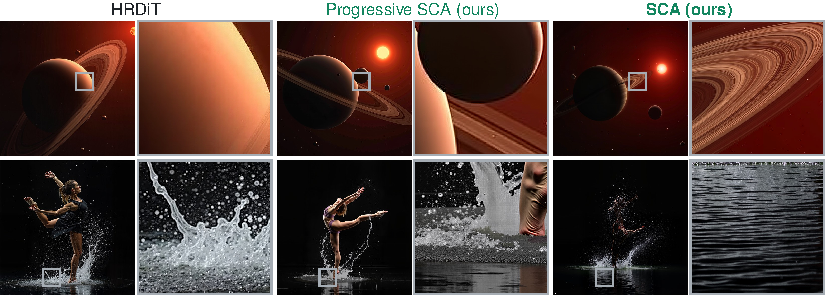
\includegraphics[width=\linewidth]{figures/progressive.pdf}
  \caption{\textbf{Progressive \sca{} (HRDiT's schedule, \sca{} attention) keeps one large subject as HRDiT does, while single-pass \sca{} can shrink or repeat subjects in these prompts.} Seed~0; two prompts drawn at random (seed~17) from the 46-prompt panel; crops are the same native ${512\times512}$ window per row, auto-placed at maximal edge energy averaged over the three methods. Times are 46-prompt campaign means (Table~\ref{tab:panel46}, Section~\ref{sec:progressive}).}
  \label{fig:progressive}
\end{figure}
